%
% 23-faktorisierung.tex
%
% (c) 2023 Prof Dr Andreas Müller

%
%
% Faktorisierung der Vandermonde-Matrix
%
\subsection{Faktorisierung der Vandermonde-Matrix
\label{buch:diskret:subsetion:faktorisierung}}
Die Fourier-Transformation $\mathscr{F}$ und ihre Inverse
$\overline{\mathscr{F}}$ sind nach
\eqref{buch:diskret:vandermonde:eqn:vanderfourier}
und
\eqref{buch:diskret:vandermonde:eqn:vanderifourier}
spezielle Van\-der\-mon\-de-Matrizen.
Zusätzlich gilt aber $\omega^n=1$ gilt.
Dies ermöglicht eine Faktorisierung der Vandermonde-Matrizen, die
im Abschnitt~\ref{buch:diskret:section:schnell} dazu verwendet
werden wird, die diskrete Fourier-Transformation deutlich schneller
als mit Hilfe der Matrizenmultiplikation mit der Matrix $\mathscr{F}$
zu berechnen.

%
% Faktorisierung im Fall n=6
%
\subsubsection{Faktorisierung im Fall $n=6$}
In diesem Abschnitt berechnen wir eine Faktorisierung der
Fourier-Transformation $\mathscr{F}_n$ für den Fall $n=6$,
die aus der Faktorisierung $n=2\cdot 3$ folgt.
Zu diesem Zweck sei $\omega^6=1$.
Die zu faktorisierende Matrix ist
\[
\mathscr{F}_6
=
\begin{pmatrix}
1&       1&          1&          1&          1&          1\\
1&  \omega&   \omega^2&   \omega^3&   \omega^4&   \omega^5\\
1&\omega^2&   \omega^4&   \omega^6&   \omega^8&\omega^{10}\\
1&\omega^3&   \omega^6&   \omega^9&\omega^{12}&\omega^{15}\\
1&\omega^4&   \omega^8&\omega^{12}&\omega^{16}&\omega^{20}\\
1&\omega^5&\omega^{10}&\omega^{15}&\omega^{20}&\omega^{25}
\end{pmatrix}
=
\begin{pmatrix}
1&       1&       1&       1&       1&       1\\
1&  \omega&\omega^2&\omega^3&\omega^4&\omega^5\\
1&\omega^2&\omega^4&       1&\omega^2&\omega^4\\
1&\omega^3&       1&\omega^3&       1&\omega^3\\
1&\omega^4&\omega^2&       1&\omega^4&\omega^2\\
1&\omega^5&\omega^4&\omega^3&\omega^2&\omega
\end{pmatrix}
\]
mit $\omega = e^{2\pi i/6}$ mit der Eigenschaft $\omega^6=1$.
Die zweite Version resultiert durch Anwendung der Identität $\omega^6=1$.

Durch Ausmultiplizieren kann man nachrechnen, dass
\[
\mathscr{F}_6
=
\underbrace{
\left(\begin{array}{ccc|ccc}
1&       1&       1&      0&       0&          0\\
0&       0&       0&      1&\omega  &   \omega^2\\
\hline
1&\omega^2&\omega^4&      0&       0&          0\\
0&       0&       0&      1&\omega^3&   \omega^6\\
\hline
1&\omega^4&\omega^6&      0&       0&          0\\
0&       0&       0&      1&\omega^5&\omega^{10}
\end{array}\right)
}_{\displaystyle =A(3,2,\omega)}
\underbrace{
\left(\begin{array}{ccc|ccc}
1&0&0&       1&       0&       0\\
0&1&0&       0&       1&       0\\
0&0&1&       0&       0&       1\\
\hline
1&0&0&\omega^3&       0&       0\\
0&1&0&       0&\omega^3&       0\\
0&0&1&       0&       0&\omega^3\\
\end{array}\right)
}_{\displaystyle =F(2,3,\omega)}
\]
Dabei muss auch wieder $\omega^6=1$ verwendet werden, zum Beispiel
bei der Berechnung der vierten Zeile, wo sich die Werte
\[
\renewcommand\arraycolsep{2pt}
\begin{array}{rclcrclcrclcrclcrclcrclcl}
0&\cdot&1 &+& 0&\cdot&0 &+& 0&\cdot&0 &+& 1&\cdot&1 &+& \omega^3&\cdot&0 &+& \omega^6&\cdot&0 &=& 1 \\
0&\cdot&0 &+& 0&\cdot&1 &+& 0&\cdot&0 &+& 1&\cdot&0 &+& \omega^3&\cdot&1 &+& \omega^6&\cdot&0 &=& \omega^3 \\
0&\cdot&0 &+& 0&\cdot&0 &+& 0&\cdot&1 &+& 1&\cdot&0 &+& \omega^3&\cdot&0 &+& \omega^6&\cdot&1 &=& \omega^6 = 1 \\
0&\cdot&1 &+& 0&\cdot&0 &+& 0&\cdot&0 &+& 1&\cdot&\omega^3 &+& \omega^3&\cdot&0 &+& \omega^6&\cdot&0 &=& \omega^3 \\
0&\cdot&0 &+& 0&\cdot&1 &+& 0&\cdot&1 &+& 1&\cdot&0 &+& \omega^3&\cdot&\omega^3 &+& \omega^6&\cdot&0 &=& \omega^6=1 \\
0&\cdot&0 &+& 0&\cdot&0 &+& 0&\cdot&0 &+& 1&\cdot&0 &+& \omega^3&\cdot&0 &+& \omega^6&\cdot&\omega^3 &=& \omega^9=\omega^3 
\end{array}
\]
ergeben.
Die Rechnung für die anderen Zeilen ist entsprechend.

Alternativ ist aber auch die Faktorisierung in die Faktoren
\[
\mathscr{F}_6
=
\underbrace{
\left(\begin{array}{cc|cc|cc}
1&       1&0&       0&0&       0\\
0&       0&1&  \omega&0&       0\\
0&       0&0&       0&1&\omega^2\\
\hline
1&\omega^3&0&       0&0&       0\\
0&       0&1&\omega^4&0&       0\\
0&       0&0&       0&1&\omega^5
\end{array}\right)
}_{\displaystyle =A(2,3,\omega)}
\underbrace{
\left(\begin{array}{cc|cc|cc}
1&0&       1&       0&       1&       0\\
0&1&       0&       1&       0&       1\\
\hline
1&0&\omega^2&       0&\omega^4&       0\\
0&1&       0&\omega^2&       0&\omega^4\\
\hline
1&0&\omega^4&       0&\omega^6&       0\\
0&1&       0&\omega^4&       0&\omega^6
\end{array}\right)
}_{\displaystyle =F(3,2,\omega)}
\]
möglich.
Durch Vertauschung von Zeilen kann man den Faktor $A(3,2,\omega)$ in die
Blockform
\[
\left(
\def\l#1{\multicolumn{1}{|c}{#1}}
\def\r#1{\multicolumn{1}{c|}{#1}}
\begin{array}{cccccc}
\cline{1-2}
\l{1}&\r{       1}&     &            &     &            \\
\l{1}&\r{\omega^3}&     &            &     &            \\
\cline{1-4}
     &            &\l{1}&\r{  \omega}&     &            \\
     &            &\l{1}&\r{\omega^4}&     &            \\
\cline{3-6}
     &            &     &            &\l{1}&\r{\omega^2}\\
     &            &     &            &\l{1}&\r{\omega^5}\\
\cline{5-6}
\end{array}
\right)
\]
bringen.
Der Block in der linken oberen Ecke ist eine Fourier-Transformation
$\mathscr{F}_2$.
Auch die anderen beiden Blöcke sind bis auf eine Multiplikation
der zweiten Spalte mit $\omega$ bzw.~$\omega^2$ Fourier-Transformationen
$\mathscr{F}_2$.

Die gleiche Art von Blockstruktur lässt sich auch für $A(3,2,\omega)$
erreichen, sie ist
\[
\left(
\def\l#1{\multicolumn{1}{|c}{#1}}
\def\r#1{\multicolumn{1}{c|}{#1}}
\begin{array}{cccccc}
\cline{1-3}
\l{1}&       1&\r{       1}&     &        &            \\
\l{1}&\omega^2&\r{\omega^4}&     &        &            \\
\l{1}&\omega^4&\r{\omega^6}&     &        &            \\
\cline{1-6}
     &        &            &\l{1}&\omega  &\r{\omega^2}\\
     &        &            &\l{1}&\omega^3&\r{\omega^6}\\
     &        &            &\l{1}&\omega^5&\r{\omega^{10}}\\
\cline{4-6}
\end{array}
\right)
\]
Die Blockmatrix in der linken oberen Ecke ist $\mathscr{F}_3$,
bis auf die Faktoren $\omega$ und $\omega^2$ in der zweiten
und dritten Spalte ist auch der Block rechts unten eine
Fourier-Transformation $\mathscr{F}_3$.

\begin{figure}
\centering
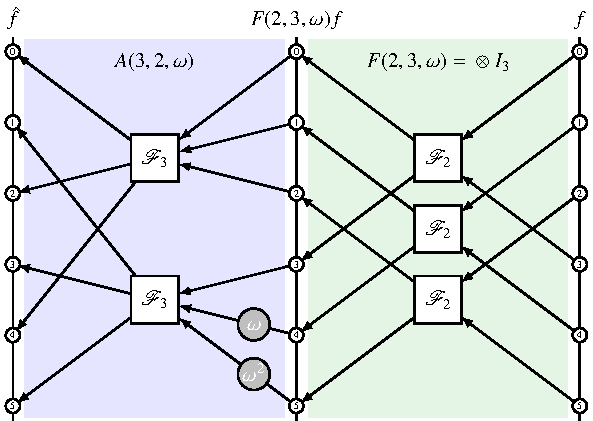
\includegraphics{chapters/060-diskret/images/f32.pdf}
\caption{Faktorisierung der Fourier-Transformation $\mathscr{F}_6$ als
$\mathscr{F}_6=A(3,2,\omega)F(2,3,\omega)$.
Die alternative Faktorisierung ist in
Abbildung~\ref{buch:diskret:faktorisierung:fig:f23}
dargestellt.
\label{buch:diskret:faktorisierung:fig:f32}}
\end{figure}
\begin{figure}
\centering
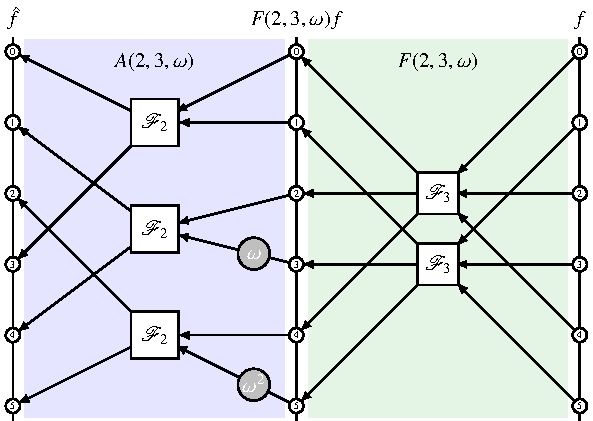
\includegraphics{chapters/060-diskret/images/f23.pdf}
\caption{Faktorisierung der Fourier-Transformation $\mathscr{F}_6$ als
$\mathscr{F}_6=A(2,3,\omega)F(3,2,\omega)$.
Die alternative Faktorisierung ist in
Abbildung~\ref{buch:diskret:faktorisierung:fig:f32}
dargestellt.
\label{buch:diskret:faktorisierung:fig:f23}}
\end{figure}

Die beiden Faktorisierungen werden in den Abbildungen
\ref{buch:diskret:faktorisierung:fig:f32}
und
\ref{buch:diskret:faktorisierung:fig:f23}
schematisch dargestellt.


%
% Rechenaufwand
%
\subsubsection{Rechenaufwand}
Die beiden Faktoren $A(p,q,\omega)$ und $F(q,p,\omega)$ enthalten
viele verschwindende Einträge.
In jeder Zeile von $A(p,q,\omega)$ sind genau $p$ Einträge von
$0$ verschieden während in jeder Zeile von $F(q,p,\omega)$ genau
$q$ Einträge von $0$ verschieden sind.
Da alle Einträge von $\mathscr{F}_6$ von Null verschieden sind, benötigt
die Berechnung des Produktes $\hat{f}=\mathscr{F}_6f$ für jede
Komponenten von $\hat{f}$ $6$ Multiplikationen und $5$ Additionen.
Für eine beliebige $n\times n$-Matrix ohne verschwindende Einträge
ist der Rechenaufwand von der Grössenordnung $O(n^2)$.

Da $A(p,q,\omega)$ und $F(q,p,\omega)$ wenige von $0$ verschiedene
Einträge haben, besteht die Möglichkeit, dass die Berechnung
von $\hat{f}=A(p,q,\omega)F(q,p,\omega)f$ mit weniger Operationen
möglich sein könnte.
Hat eine $n\times n$-Matrix $A$ auf jeder Zeile genau $m$ von $0$
verschiedene Einträge, dann sind zur Berechnung des Produktes $Ax$
für jede Zeile genau $m$ Multiplikationen und $m-1$ Additionen
nötig.
Die Berechnung von $Ax$ ist also mit $nm$ Multiplikationen und 
$n(m-1)$ Additionen möglich.
Für $A(p,q,\omega)$ ist $m=q$ und für $F(p,q,\omega)$ ist $m=p$.
Die Berechnung von des Produktes ist daher mit
\begin{align*}
&n(q+p)\text{ Multiplikationen}
\\
&n(q+p-2)\text{ Additionen}
\end{align*}
möglich.
Da $p+q=5<6=n=pq$ ist, verringert die Faktorisierung den Rechenaufwand
tatsächlich um etwa 16\%.
Dies ist zwar nicht viel, aber in Abschnitt~\ref{buch:diskret:section:schnell}
werden wir zeigen, wie diese Idee dazu verwendet werden kann, die
Fourier-Transformation für geeignet gewählte Dimensionen $n$ auf
$O(n\log n)$ zu reduzieren.

